\chapter{Survey of the state-of-the-art LPs}
\label{chapter3}

\section{Table of profiles}

While in related work we examined load profiling in general,
this chapter focuses on how data in load profiles is presented.  
It can be portrayed in various shapes and forms,
using all kinds of attributes and features to do so. 
First, main load profiling features will be defined.
Second, using these features a general load profile table will be constructed.
Third, references from related work and use cases will be mapped to the table.
Using this information main features will be selected.
Fourth, using a reduced feature set a more detailed table will be formed.
Again, the table will be populated using the same references as before.
Finally, using this information a research direction will be formed.

\subsection{Feature set} \label{sec:feature_set}

Using related work from this chapter and use-case references from chapter \ref{chapter4},
we can extract the most commonly used features to portray load profiles.

\begin{outline}
    \1 power
    \1 time
    \1 operating time (how long appliance or appliances is turned on)
    \1 appliances (a set)
    \1 Number of activations (How many times appliance or appliances were turned on)
\end{outline}

\subsection{General table}
Using these features we can form a table with all possible combinations.
Some combinations do not make logical sense and the others repeat themselves.
Such examples are marked with the letter X.
Table \ref{tab:general_map} is then populated with references from previous chapters.

To understand the table clearer, let's imagine that each feature is used as an axis label when plotting. 
That is for example why we did not use only the power consumption feature, but three variations of it. 
The first one is average power usage. It is an integer, and it could be an average of hourly, daily or yearly consumption. 
The next possibility is an array where we use a set of integers in any combination.
Finally, we have a histogram that is obtained from the power time array. 

\begin{table}[H]
    \caption{General table of load profiles}
    \label{tab:general_map}
    \begin{tabular}{|c|c|c|c|c|c|}
    \hline
        &
        frequency &
        appliances &
        \begin{tabular}[c]{@{}l@{}}number of\\ activations\end{tabular} &
        \begin{tabular}[c]{@{}l@{}}power\\ (avg)\end{tabular} &
        \begin{tabular}[c]{@{}l@{}}operating\\ time\end{tabular} \\ \hline
    appliances                                                      &   & X & X & X  & X    \\ \hline
    \begin{tabular}[c]{@{}c@{}}number of\\ activations\end{tabular} & X & \multicolumn{1}{c|}{\begin{tabular}[c]{@{}c@{}} \citeyear*{per_appliance_per_building} \\ \citeyear*{UKDALE} \end{tabular}} & X & X  & X    \\ \hline
    \begin{tabular}[c]{@{}c@{}}power \\ (avg)\end{tabular}          & X & \citeyear*{appliance_avgpower} &   & X  & X    \\ \hline
    \begin{tabular}[c]{@{}c@{}}power \\ (array)\end{tabular}        & \citeyear*{UKDALE} & X & X & X  & X    \\ \hline
    \begin{tabular}[c]{@{}c@{}}power \\ (histogram)\end{tabular}    &   &   & X & X  & X    \\ \hline
    \begin{tabular}[c]{@{}c@{}}operating\\ time\end{tabular}        & X & \citeyear*{operating_time} & \multicolumn{1}{c|}{\begin{tabular}[c]{@{}c@{}} \citeyear*{NILMAD2019} \\ \citeyear*{NILMAD22019} \\ \citeyear*{NILMAD2021} \end{tabular}} &  \citeyear*{NILMAD2021} & X    \\ \hline
    time array                                                      & X & X & \multicolumn{1}{c|}{\begin{tabular}[c]{@{}c@{}} \citeyear*{per_appliance_per_building} \\ \citeyear*{UKDALE} \end{tabular}} &  \multicolumn{1}{c|}{\begin{tabular}[c]{@{}c@{}} \citeyear*{Chuan2014} \\ \citeyear*{Csoknyai2019} \\ \citeyear*{H0} \\ \citeyear*{KAVOUSIAN2013184} \\ \citeyear*{WALKER1985} \\ 	\citeyear*{GERBEC2005} \\ 	\citeyear*{Gao2018} \\ 	\citeyear*{Jeong2021}\\  	\citeyear*{Joana2012} \\ 	\citeyear*{DER_heatmap_profile}\\ 	\citeyear*{NILMAD2019}\\	\citeyear*{NILMAD22019} \\	\citeyear*{Issi2018} \\	\citeyear*{NILMAD2021}\\	\citeyear*{Castangia2021} \\	\citeyear*{occupancy2013} \\	\citeyear*{Chuan2014} \\ 	\citeyear*{CAPASSO1994} \\ 	\citeyear*{Park2019} \\	\citeyear*{UKDALE} \\	\citeyear*{Gao2018} \end{tabular}}    & \citeyear*{OperatingTime_timeofday} \\ \hline
    \end{tabular}
\end{table}

The first profile is the one in the first row and the first column.
It is a combination of frequency and appliances. 
This would mean that we would have appliances on the x-axis and the number of occurrences o the y-axis.
The only useful application for this profile is when presenting how many appliances of one type are in one dataset. 
Other than that it has no use-cases and that is probably the reason why it is rarely used.

The next possible combination is between a number of activations and appliances. 
Here the explanation is relatively straightforward. The combination shows us how many times each appliance activities.

The second presentation of data is a combination of power and number of activations. 
In this case, we would construct a histogram of power values. 
On the x-axis we would have power values on the y-Axis we would have a number of times this power value occurred, where we would have buckets of a certain size.
Here we should not mix it up with the previous combination, since here we include the whole consumption and not only when turned on. 

The combination in the second column and second row is between average power, an integer, and appliances. Again explanation is simple. We present the average consumption for each appliance in a household.

The combination in the third column and second row, between average power and numbers of activations, is again less straightforward.
It presents how many times it activated with a certain power.

Here one feature is an output of the previous combination, a histogram of power. 
It is possible to have a histogram of the histogram, but it is not practical. 
This means we are looking at looking how many times did the occurrence occur. 
Not all combinations, even though they are possible, are useful. 

The combination in the second column and fifth row is again straightforward. 
Plotting histograms for each appliance and then plotting them side by side.
In this case, we present histograms in color, since we are working with 3 dimensions.

In the case of combining the second column and sixth row, between appliances and operating time, we present how long each appliance operates.
Here it could be either a number or even a time range presentation.
When doing a combination between operating time and the number of activations we are plotting how many times did an appliance turn on for a certain amount of time

In the case of a combination between operating time and power, we show how long did appliance operate with a certain power.

Next case, in the third row and last column, a combination between time array and several activations we present when did appliance turn on certain amount of times. 

We are coming to an end, and here we have the most commonly used case where we use time array and average power to present the data.

In the final case, the combination shows us at which time do appliance operate for a certain amount of time 

Based on table \ref{tab:general_map} it is possible to see that the most commonly
published feature combination is time and power. This combination will be used 
as a baseline when making a more detailed table. Although the operating time feature was 
explored in a few publications a bit, and it seems quite promising, we are 
focusing on activation-based histogram representation.
Based on table \ref{tab:general_map} it is possible to see that not much attention was given to it. 

\subsection{Detailed table}

This section will focus on exploring possible load profiles using activation-based histogram representation,
while using the power feature as a baseload. 
Features from \ref{tab:general_map} will be explored in higher detail. 
They will be split and arranged in a way that all 21 publications and power-based presentations will be divided into as many groups as possible. 
This should expose possible activation-based profiles as well as unpublished power-based profiles.

\subsubsection{Sub-features} \label{sec:subfeatures}

Main features were already described in section \ref{sec:feature_set}.
It is possible to further divide them into smaller so-called sub-features.
These are reshaped and grouped as follows:
\begin{outline}

\1 Way of presenting a profile
\2 Per-building load profile
\2 Per-appliance load profiles
\2 Per-building and per appliance load profile

\1 By time range of profile 
\2 Daily
\2 Weekly
\2 Monthly
\2 Yearly

\1 Way of measuring usage
\2 Average power use 
\2 Activation or frequency of activation
\end{outline}


\subsection{Table of combinations or detailed table}

The above-shown profiles can be combined, yielding a new way of displaying the data.
Bellow, a map with combinations of the above-mentioned profiles is presented. 
The purpose of table \ref{fig:map_fig} to generate and show possible combinations.
Some combinations that had similar output were grouped, and some that could not be sketched were discarded. 

\begin{figure}[H]
	\centering
	\caption{"Table of combinations"}
	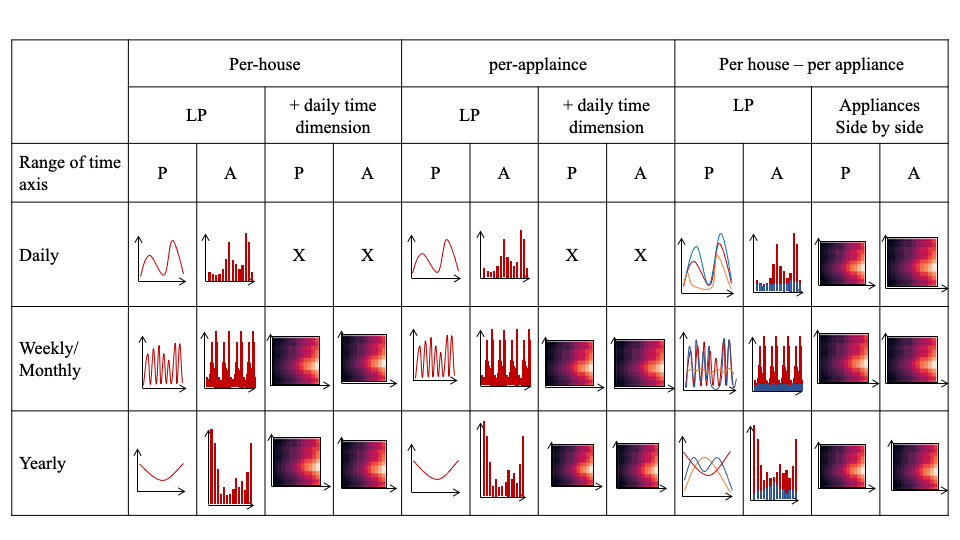
\includegraphics[width=0.9\textwidth]{Figures/profile_sketches/Slide14.png}
	\label{fig:map_fig}
\end{figure}

Figure above \ref{fig:map_fig}, uses sub-features from previous subsection \ref{sec:subfeatures}. 
In general, the table is formatted in a way that features from columns are
used in the x-axis of a plot, and rows are used in the y or z-axis of a plot. 

The column of the table presents the time domain. "Daily" means that the load profile presents
average usage for one day, weekly means it presents usage for a week.
To be clear, for one to construct a decent daily profile, one needs a few
weeks of data. The same goes for yearly profiles, in that case, one needs many years' worth of data. 

The top row of the table is composed of 3 main groups. 
The first group focuses on Per-building energy consumption.
The second group examines the energy consumption of each appliance in a house separately.
Third group analyses all appliances in a building.

The next row of the table is further divided into two groups. First is the profile group
which presents the given usage unit on the y-axis and time on the x-axis. 
Next is a profile with a time group. 
In this case, we present the given usage unit on the z-axis and then time on the x and y-axis.
Here, the second-time dimension can be anything from a week to a year.
In the case of the Per-building subgroup includes appliances instead of time. 
Example for this is figure \ref{fig:heatmap_all_appl}.
The last columns present the usage unit, that is power (P) or a number of activations (A).

\subsection{Mapping references to the table of profiles}

To find useful load profiles, references from related work must be mapped.

\begin{table}[H]
	\caption{Table presents previously mentioned load profiles}
	\label{tab:contributions}
	\begin{tabular}{|l|cccc|cccc|cccc|}
	\hline
	Description                                                   & \multicolumn{4}{c|}{Per-building}                                                                                               & \multicolumn{4}{c|}{Per-appliance}                                                                                           & \multicolumn{4}{c|}{\begin{tabular}[c]{@{}c@{}}Per-building\\ per-appliance\end{tabular}}                                                         \\ \hline
																 & \multicolumn{2}{c|}{LP}                         & \multicolumn{2}{c|}{\begin{tabular}[c]{@{}c@{}} + daily time \\ dimension \end{tabular}} & \multicolumn{2}{c|}{LP}                         & \multicolumn{2}{c|}{\begin{tabular}[c]{@{}c@{}} + daily time \\ dimension \end{tabular}} & \multicolumn{2}{c|}{LP}                               & \multicolumn{2}{c|}{\begin{tabular}[c]{@{}c@{}}Appliances\\ side by side\end{tabular}} \\ \hline
	\begin{tabular}[c]{@{}l@{}}Range of time\\ axis\end{tabular} & \multicolumn{1}{c|}{P} & \multicolumn{1}{c|}{A} & \multicolumn{1}{c|}{P}                         & A                         & \multicolumn{1}{c|}{P} & \multicolumn{1}{c|}{A} & \multicolumn{1}{c|}{P}                         & A                         & \multicolumn{1}{c|}{P}    & \multicolumn{1}{c|}{A}    & \multicolumn{1}{c|}{P}                               & A                               \\ \hline
	Daily                                                        & \multicolumn{1}{c|}{\begin{tabular}[c]{@{}c@{}} \citeyear*{UKDALE} \\ \citeyear*{Chuan2014} \\ \citeyear*{Csoknyai2019} \\ \citeyear*{H0} \\ \citeyear*{KAVOUSIAN2013184} \\ \citeyear*{CAPASSO1994} \\ \citeyear*{WALKER1985} \\ \citeyear*{GERBEC2005} \\ \citeyear*{Gao2018} \\ \citeyear*{Jeong2021} \\ \citeyear*{Joana2012} \\ \citeyear*{DER_heatmap_profile} \end{tabular}}  & \multicolumn{1}{c|}{}  & \multicolumn{1}{c|}{X}  &  X  & \multicolumn{1}{c|}{\begin{tabular}[c]{@{}l@{}} \citeyear*{NILMAD2019} \\ \citeyear*{NILMAD22019} \\ \citeyear*{Issi2018} \\ \citeyear*{NILMAD2021} \\ \citeyear*{Castangia2021} \\ \citeyear*{occupancy2013}	\end{tabular}}  & \multicolumn{1}{c|}{\citeyear*{UKDALE}}  & \multicolumn{1}{c|}{X}   &  \multicolumn{1}{c|}{X}   & \multicolumn{1}{c|}{\begin{tabular}[c]{@{}l@{}} \citeyear*{Chuan2014} \\ \citeyear*{CAPASSO1994} \\ \citeyear*{Gao2018} 	\end{tabular}}   & \multicolumn{1}{c|}{\citeyear*{UKDALE}}     & \multicolumn{1}{c|}{}      &    \\ \hline
	\begin{tabular}[c]{@{}l@{}}Weekly/\\ Monthly\end{tabular}    & \multicolumn{1}{c|}{\begin{tabular}[c]{@{}c@{}} \citeyear*{Csoknyai2019} \\ \citeyear*{H0} \\ \citeyear*{KAVOUSIAN2013184} \end{tabular}}  & \multicolumn{1}{c|}{}  & \multicolumn{1}{c|}{\begin{tabular}[c]{@{}l@{}} \citeyear*{2D_year_day_LP} \\ \citeyear*{Park2019} \\ \citeyear*{DER_heatmap_profile} \end{tabular}}                            &                           & \multicolumn{1}{c|}{}  & \multicolumn{1}{c|}{\citeyear*{per_appliance_per_building}}  & \multicolumn{1}{c|}{}                          &                           & \multicolumn{1}{c|}{\citeyear*{weekly_per_appliance_LP}}    & \multicolumn{1}{c|}{\citeyear*{per_appliance_per_building}}     & \multicolumn{1}{c|}{}                                &                                 \\ \hline
	Yearly                                                       & \multicolumn{1}{c|}{\begin{tabular}[c]{@{}c@{}} \citeyear*{Csoknyai2019} \\ \citeyear*{H0} \\ \citeyear*{KAVOUSIAN2013184} \end{tabular}}  & \multicolumn{1}{c|}{}  & \multicolumn{1}{c|}{}                          &                           & \multicolumn{1}{c|}{}  & \multicolumn{1}{c|}{}  & \multicolumn{1}{c|}{}                          &                           & \multicolumn{1}{c|}{}     & \multicolumn{1}{c|}{}     & \multicolumn{1}{c|}{}                                &                                 \\ \hline
	\end{tabular}
\end{table}

As can be seen from table \ref{tab:contributions}, most of the work (14 publications) has been done with standard daily load profiles with
Per-building power usage such as figure \ref{fig:daily_power_profile}. 
Quite a lot of work (6 publications) has been done with per appliance daily power profiles.
A few publications were based on weekly and yearly load profiles,
and a few used two-dimensional time and power presentations.
Only one publication found used activation and time-based histogram such as 
shown in figure \ref{fig:daily_act_profile}. During the research we focused on publications
from minority classes, meaning not all existing publications for standard load profiles are included. 
The purpose of table \ref{tab:contributions} is to present missing scientific contributions and patterns of publications.  

\newcommand{\tabVar}{+ daily time \\ dimension  }
%\testIt

\subsection{Mapping use-cases to the table of combinations}

Table \ref{tab:use_cases} includes arranged publications from chapter \ref{Chapter5}. 
Similar pattern emerged as in table \ref{tab:contributions}. 

\begin{table}[H]
	\caption{Table presents references mentioned in use cases chapter}
	\label{tab:use_cases}
	\begin{tabular}{|l|cccc|cccc|cccc|}
	\hline
	Description &
	  \multicolumn{4}{c|}{Per-building} &
	  \multicolumn{4}{c|}{Per-appliance} &
	  \multicolumn{4}{c|}{\begin{tabular}[c]{@{}c@{}}Per-building\\ per-appliance\end{tabular}} \\  \hline
	  &
	  \multicolumn{2}{c|}{LP} &
	  \multicolumn{2}{c|}{\begin{tabular}[c]{@{}c@{}} \tabVar \end{tabular}} &
	  \multicolumn{2}{c|}{LP} &
	  \multicolumn{2}{c|}{\begin{tabular}[c]{@{}c@{}} \tabVar \end{tabular}} &
	  \multicolumn{2}{c|}{LP} &
	  \multicolumn{2}{c|}{\begin{tabular}[c]{@{}c@{}}Appliances\\ side by side\end{tabular}} \\ \hline
	\begin{tabular}[c]{@{}l@{}}Range of time\\ axis\end{tabular} &
	  \multicolumn{1}{c|}{P} &
	  \multicolumn{1}{c|}{A} &
	  \multicolumn{1}{c|}{P} &
	  A &
	  \multicolumn{1}{c|}{P} &
	  \multicolumn{1}{c|}{A} &
	  \multicolumn{1}{c|}{P} &
	  A &
	  \multicolumn{1}{c|}{P} &
	  \multicolumn{1}{c|}{A} &
	  \multicolumn{1}{c|}{P} &
	  A \\ \hline
	Daily &
	  \multicolumn{1}{c|}{\begin{tabular}[c]{@{}c@{}} \citeyear*{energy_saving1} \\ \citeyear*{energy_saving3} \\ \citeyear*{EV2020} \\ \citeyear*{energyStealing2018} \\ \citeyear*{shift2015} \\ \citeyear*{optimiseCostShift2015} \\ \citeyear*{controll2014} \end{tabular}} &
	  \multicolumn{1}{c|}{} &
	  \multicolumn{1}{c|}{X} &
    X
	   &
	  \multicolumn{1}{c|}{\begin{tabular}[c]{@{}c@{}} \citeyear*{EV2020} \\ \citeyear*{elder1} \\ \citeyear*{elder2} \\   \citeyear*{occupancy2013}	  \end{tabular}} &
	  \multicolumn{1}{c|}{} &
	  \multicolumn{1}{c|}{X} &
    X
	   &
	  \multicolumn{1}{c|}{\citeyear*{Chuan2014}	 } &
	  \multicolumn{1}{c|}{} &
	  \multicolumn{1}{c|}{} &
	   \\ \hline
	\begin{tabular}[c]{@{}l@{}}Weekly/\\ Monthly\end{tabular} &
	  \multicolumn{1}{c|}{\begin{tabular}[c]{@{}c@{}} \citeyear*{energy_saving3} \\ \citeyear*{KAVOUSIAN2013184}  \end{tabular}} &
	  \multicolumn{1}{c|}{} &
	  \multicolumn{1}{c|}{} &
	   &
	  \multicolumn{1}{c|}{} &
	  \multicolumn{1}{c|}{} &
	  \multicolumn{1}{c|}{} &
	   &
	  \multicolumn{1}{c|}{} &
	  \multicolumn{1}{c|}{} &
	  \multicolumn{1}{c|}{} &
	   \\ \hline
	Yearly &
	  \multicolumn{1}{c|}{\begin{tabular}[c]{@{}c@{}}\citeyear*{energy_saving3}\end{tabular}} &
	  \multicolumn{1}{c|}{} &
	  \multicolumn{1}{c|}{} &
	   &
	  \multicolumn{1}{c|}{} &
	  \multicolumn{1}{c|}{} &
	  \multicolumn{1}{c|}{} &
	   &
	  \multicolumn{1}{c|}{} &
	  \multicolumn{1}{c|}{} &
	  \multicolumn{1}{c|}{} &
	   \\ \hline
	\end{tabular}
\end{table}

\subsection{Table of use case groups}

The table \ref{tab:groups} presents same publications as \ref{tab:use_cases},
but only group names are shown.
The table indicates how groups are arranged.
Where anomaly detection and elderly care are dominating in the per-appliance part of the table,
zero energy buildings and demand response are dominating in a per-building part of the table. 

\begin{table}[H]
    \caption{Table presents references mentioned in use cases chapter}
	\label{tab:groups}
    \begin{adjustbox}{width=1.2\textwidth,center=\textwidth} 
        \begin{tabular}{|l|cccc|cccc|cccc|}
            \hline
            \begin{tabular}[c]{@{}l@{}}ZEB - zero energy buldings\\ DR - demand response\\ AD - anomaly detection\\ EC - elderly care\\ X - unfeasible\end{tabular} &
              \multicolumn{4}{c|}{Per-building} &
              \multicolumn{4}{c|}{Per-appliance} &
              \multicolumn{4}{c|}{\begin{tabular}[c]{@{}c@{}}Per-building\\ per-appliance\end{tabular}} \\ \cline{2-13} 
             &
              \multicolumn{2}{c|}{LP} &
              \multicolumn{2}{c|}{\begin{tabular}[c]{@{}c@{}}+ daily time \\ dimension\end{tabular}} &
              \multicolumn{2}{c|}{LP} &
              \multicolumn{2}{c|}{\begin{tabular}[c]{@{}c@{}} \tabVar \end{tabular}} &
              \multicolumn{2}{c|}{LP} &
              \multicolumn{2}{c|}{\begin{tabular}[c]{@{}c@{}}Appliances\\ side by side\end{tabular}} \\ \hline
            \begin{tabular}[c]{@{}l@{}}Range of time\\ axis\end{tabular} &
              \multicolumn{1}{c|}{P} &
              \multicolumn{1}{c|}{A} &
              \multicolumn{1}{c|}{P} &
              A &
              \multicolumn{1}{c|}{P} &
              \multicolumn{1}{c|}{A} &
              \multicolumn{1}{c|}{P} &
              A &
              \multicolumn{1}{c|}{P} &
              \multicolumn{1}{c|}{A} &
              \multicolumn{1}{c|}{P} &
              A \\ \hline
            Daily &
              \multicolumn{1}{c|}{ZEB, DR} &
              \multicolumn{1}{c|}{} &
              \multicolumn{1}{c|}{X} &
              X
               &
              \multicolumn{1}{c|}{\begin{tabular}[c]{@{}c@{}}AD, EC,\\ ZEB\end{tabular}} &
              \multicolumn{1}{c|}{} &
              \multicolumn{1}{c|}{X} &
              X
               &
              \multicolumn{1}{c|}{DR} &
              \multicolumn{1}{c|}{} &
              \multicolumn{1}{c|}{} &
               \\ \hline
            \begin{tabular}[c]{@{}l@{}}Weekly/\\ Monthly\end{tabular} &
              \multicolumn{1}{c|}{ZEB} &
              \multicolumn{1}{c|}{} &
              \multicolumn{1}{c|}{} &
               &
              \multicolumn{1}{c|}{} &
              \multicolumn{1}{c|}{} &
              \multicolumn{1}{c|}{} &
               &
              \multicolumn{1}{c|}{} &
              \multicolumn{1}{c|}{} &
              \multicolumn{1}{c|}{} &
               \\ \hline
            Yearly &
              \multicolumn{1}{c|}{ZEB} &
              \multicolumn{1}{c|}{} &
              \multicolumn{1}{c|}{} &
               &
              \multicolumn{1}{c|}{} &
              \multicolumn{1}{c|}{} &
              \multicolumn{1}{c|}{} &
               &
              \multicolumn{1}{c|}{} &
              \multicolumn{1}{c|}{} &
              \multicolumn{1}{c|}{} &
               \\ \hline
            \end{tabular}
    \end{adjustbox} 
    \end{table}

The figures listed above clearly depict the void not filled by publications. 
Although they may not be published, they still have a possible use case. 
In table \ref{tab:groups_proposed} empty spaces are filled 
with possible use cases for given load profiles. 

\begin{table}[H]
    \caption{"Proposed use cases for profiles"}
    \label{tab:groups_proposed}
    \begin{adjustbox}{width=1.2\textwidth,center=\textwidth} 
    \begin{tabular}{|l|cccc|cccc|cccc|}
    \hline
    \begin{tabular}[c]{@{}l@{}}ZEB - zero energy buildings\\ DR - demand response\\ AD - anomaly detection\\ EC - elderly care\\ X - unfeasible\end{tabular} &
      \multicolumn{4}{c|}{Per-building} &
      \multicolumn{4}{c|}{Per-appliance} &
      \multicolumn{4}{c|}{\begin{tabular}[c]{@{}c@{}}Per-building\\ per-appliance\end{tabular}} \\ \cline{2-13} 
     &
      \multicolumn{2}{c|}{LP} &
      \multicolumn{2}{c|}{\begin{tabular}[c]{@{}c@{}}+ daily time \\ dimension\end{tabular}} &
      \multicolumn{2}{c|}{LP} &
      \multicolumn{2}{c|}{\begin{tabular}[c]{@{}c@{}} \tabVar \end{tabular}} &
      \multicolumn{2}{c|}{LP} &
      \multicolumn{2}{c|}{\begin{tabular}[c]{@{}c@{}}Appliances\\ side by side\end{tabular}} \\ \hline
    \begin{tabular}[c]{@{}l@{}}Range of time\\ axis\end{tabular} &
      \multicolumn{1}{c|}{P} &
      \multicolumn{1}{c|}{A} &
      \multicolumn{1}{c|}{P} &
      A &
      \multicolumn{1}{c|}{P} &
      \multicolumn{1}{c|}{A} &
      \multicolumn{1}{c|}{P} &
      A &
      \multicolumn{1}{c|}{P} &
      \multicolumn{1}{c|}{A} &
      \multicolumn{1}{c|}{P} &
      A \\ \hline
    Daily &
      \multicolumn{1}{c|}{\begin{tabular}[c]{@{}c@{}}AD,\\ ZEB, DR,\end{tabular}} &
      \multicolumn{1}{c|}{\begin{tabular}[c]{@{}c@{}}AD,\\ ZEB, DR,\end{tabular}} &
      \multicolumn{1}{c|}{X} &
      X &
      \multicolumn{1}{c|}{\begin{tabular}[c]{@{}c@{}}AD, EC,\\ ZEB, DR\end{tabular}} &
      \multicolumn{1}{c|}{\begin{tabular}[c]{@{}c@{}}AD, EC,\\ ZEB, DR\end{tabular}} &
      \multicolumn{1}{c|}{\begin{tabular}[c]{@{}c@{}} X \end{tabular}} &
      \begin{tabular}[c]{@{}c@{}} X \end{tabular} &
      \multicolumn{1}{c|}{\begin{tabular}[c]{@{}c@{}}AD, EC,\\ ZEB, DR\end{tabular}} &
      \multicolumn{1}{c|}{\begin{tabular}[c]{@{}c@{}}AD, EC,\\ ZEB, DR\end{tabular}} &
      \multicolumn{1}{c|}{\begin{tabular}[c]{@{}c@{}}AD, EC,\\ ZEB, DR\end{tabular}} &
      \begin{tabular}[c]{@{}c@{}}AD, EC,\\ ZEB, DR\end{tabular} \\ \hline
    \begin{tabular}[c]{@{}l@{}}Weekly/\\ Monthly\end{tabular} &
      \multicolumn{1}{c|}{\begin{tabular}[c]{@{}c@{}}AD,\\ ZEB, DR\end{tabular}} &
      \multicolumn{1}{c|}{\begin{tabular}[c]{@{}c@{}}AD,\\ ZEB, DR,\end{tabular}} &
      \multicolumn{1}{c|}{ZEB, DR} &
      ZEB, DR &
      \multicolumn{1}{c|}{\begin{tabular}[c]{@{}c@{}}AD,\\ ZEB, DR\end{tabular}} &
      \multicolumn{1}{c|}{\begin{tabular}[c]{@{}c@{}}AD,\\ ZEB, DR\end{tabular}} &
      \multicolumn{1}{c|}{\begin{tabular}[c]{@{}c@{}}AD,\\ ZEB, DR\end{tabular}} &
      \begin{tabular}[c]{@{}c@{}}AD,\\ ZEB, DR\end{tabular} &
      \multicolumn{1}{c|}{\begin{tabular}[c]{@{}c@{}}AD,\\ ZEB, DR\end{tabular}} &
      \multicolumn{1}{c|}{\begin{tabular}[c]{@{}c@{}}AD,\\ ZEB, DR\end{tabular}} &
      \multicolumn{1}{c|}{\begin{tabular}[c]{@{}c@{}}AD,\\ ZEB, DR\end{tabular}} &
      \begin{tabular}[c]{@{}c@{}}AD,\\ ZEB, DR\end{tabular} \\ \hline
    Yearly &
      \multicolumn{1}{c|}{ZEB, DR} &
      \multicolumn{1}{c|}{ZEB, DR} &
      \multicolumn{1}{c|}{ZEB, DR} &
      ZEB, DR &
      \multicolumn{1}{c|}{\begin{tabular}[c]{@{}c@{}}AD,\\ ZEB, DR\end{tabular}} &
      \multicolumn{1}{c|}{\begin{tabular}[c]{@{}c@{}}AD,\\ ZEB, DR\end{tabular}} &
      \multicolumn{1}{c|}{ ZEB, DR } &
      ZEB, DR &
      \multicolumn{1}{c|}{ZEB,DR}  &
      \multicolumn{1}{c|}{\begin{tabular}[c]{@{}c@{}}AD,\\ ZEB, DR\end{tabular}} &
      \multicolumn{1}{c|}{\begin{tabular}[c]{@{}c@{}}AD,\\ ZEB, DR\end{tabular}} &
      \begin{tabular}[c]{@{}c@{}}AD,\\ ZEB, DR\end{tabular} \\ \hline
    \end{tabular}
    \end{adjustbox}
\end{table}

\subsection{Table of load profile potentials} \label{subsec:potential}

Some combinations are indeed illogical and again others are less useful in a practical sense.
The next table will try to rate the scientific potential of the profiles based on two characteristics. 
First is how well data is presented to the user,
meaning that the load profile is clear at what it is presenting.
The second is the effectiveness when being used in an algorithm, or in other words, how well data is presented to a machine. 
These characteristics can not be easily measured,
but it is possible to extract them based on the pattern of publications.
To do that, we have to make two assumptions.
The first one would be, that the larger the number of publications, the larger is the effectiveness of presenting the data to a human.
The second would be, that the larger the number of use cases, the better the effectiveness of presenting the data to a machine.
Using these two assumptions, we propose the following table. 
The table has four possible classes. 

\begin{outline} 
\1 1 - The load profile satisfies both assumptions and has a high utility rate and was already researched (high research potential). 
\1 2 - The load profile satisfies only one of the above-mentioned assumptions (mid-research potential).
\1 3 - The load profile does not suffice any of the above-mentioned assumptions and was not yet researched or practically used (low research potential).
\1 X - The load profile is inexplicable.
\end{outline}

\begin{table}[H]
    \caption{Proposed classification of profiles}
    \label{tab:classified_profiles}
    \begin{tabular}{|l|cccc|cccc|cccc|}
    \hline
     &
      \multicolumn{4}{c|}{Per-building} &
      \multicolumn{4}{c|}{Per-appliance} &
      \multicolumn{4}{c|}{\begin{tabular}[c]{@{}c@{}}Per-building\\ per-appliance\end{tabular}} \\ \cline{2-13} 
     &
      \multicolumn{2}{c|}{LP} &
      \multicolumn{2}{c|}{\begin{tabular}[c]{@{}c@{}}+ daily time \\ dimension\end{tabular}} &
      \multicolumn{2}{c|}{LP} &
      \multicolumn{2}{c|}{\begin{tabular}[c]{@{}c@{}} \tabVar \end{tabular}} &
      \multicolumn{2}{c|}{LP} &
      \multicolumn{2}{c|}{\begin{tabular}[c]{@{}c@{}}Appliances\\ side by side\end{tabular}} \\ \hline
    \begin{tabular}[c]{@{}l@{}}Range of time\\ axis\end{tabular} &
      \multicolumn{1}{c|}{P} &
      \multicolumn{1}{c|}{A} &
      \multicolumn{1}{c|}{P} &
      A &
      \multicolumn{1}{c|}{P} &
      \multicolumn{1}{c|}{A} &
      \multicolumn{1}{c|}{P} &
      A &
      \multicolumn{1}{c|}{P} &
      \multicolumn{1}{c|}{A} &
      \multicolumn{1}{c|}{P} &
      A \\ \hline
    Daily &
      \multicolumn{1}{c|}{1} &
      \multicolumn{1}{c|}{3} &
      \multicolumn{1}{c|}{X} &
      X &
      \multicolumn{1}{c|}{1} &
      \multicolumn{1}{c|}{2} &
      \multicolumn{1}{c|}{X} &
      X &
      \multicolumn{1}{c|}{1} &
      \multicolumn{1}{c|}{2} &
      \multicolumn{1}{c|}{3} &
      3 \\ \hline
    \begin{tabular}[c]{@{}l@{}}Weekly/\\ Monthly\end{tabular} &
      \multicolumn{1}{c|}{1} &
      \multicolumn{1}{c|}{3} &
      \multicolumn{1}{c|}{2} &
      3 &
      \multicolumn{1}{c|}{3} &
      \multicolumn{1}{c|}{2} &
      \multicolumn{1}{c|}{3} &
      3 &
      \multicolumn{1}{c|}{2} &
      \multicolumn{1}{c|}{2} &
      \multicolumn{1}{c|}{3} &
      3 \\ \hline
    Yearly &
      \multicolumn{1}{c|}{1} &
      \multicolumn{1}{c|}{3} &
      \multicolumn{1}{c|}{3} &
      3 &
      \multicolumn{1}{c|}{3} &
      \multicolumn{1}{c|}{3} &
      \multicolumn{1}{c|}{3} &
      3 &
      \multicolumn{1}{c|}{3} &
      \multicolumn{1}{c|}{3} &
      \multicolumn{1}{c|}{3} &
      3 \\ \hline
    \end{tabular}
\end{table}

\subsection{Table of possible future research directions}

The table \ref{tab:classified_profiles} shows which profiles were researched and which were not yet.
To find future research directions we must look into profiles that were least researched.
These profiles are marked with the number 3 on table \ref{tab:classified_profiles}.
Some profiles were not researched because they may not present data as well,
and some were simply overlooked. 

This is why we have built the following table \ref{tab:future_rd}.
The table was marked as follows:

\begin{outline} 
\1 (1) - The load profile has high potential. 
\1 (2) - The load profile has mid-potential.
\1 Empty - The load profile has low potential or was already researched.
\1 X - load profile is inexplicable
\end{outline}

The process of evaluation was a bit complicated, but it can be summed down to the following rules.

If the load profile was used as a power profile, can it be used as an activation profile?
Here we must use some common sense since per-building power load profiles were commonly used and based on that activation load profiles should be useful as well.
That is not the case since to build per-building activation load profiles we need per-appliance (sub-meter) data anyway. That is why we have assigned them to the second class.

Another rule that was followed was useful for combined load profiles, such as 2D time profiles. 
If one dimension of load profiles was used, with what other dimension could it be combined?
In the case where one dimension was commonly used, it is probably worth investigating it with a combination of additional dimensions. 

Following these rules, the table  \ref{tab:future_rd} was constructed.


\begin{table}[H]
    \caption{Possible future research contributions}
    \label{tab:future_rd}
    \begin{tabular}{|l|cccc|cccc|cccc|}
    \hline
     &
      \multicolumn{4}{c|}{Per-building} &
      \multicolumn{4}{c|}{Per-appliance} &
      \multicolumn{4}{c|}{\begin{tabular}[c]{@{}c@{}}Per-building\\ per-appliance\end{tabular}} \\ \cline{2-13} 
     &
      \multicolumn{2}{c|}{LP} &
      \multicolumn{2}{c|}{\begin{tabular}[c]{@{}c@{}}+ daily time \\ dimension\end{tabular}} &
      \multicolumn{2}{c|}{LP} &
      \multicolumn{2}{c|}{\begin{tabular}[c]{@{}c@{}} \tabVar \end{tabular}} &
      \multicolumn{2}{c|}{LP} &
      \multicolumn{2}{c|}{\begin{tabular}[c]{@{}c@{}}Appliances\\ side by side\end{tabular}} \\ \hline
    \begin{tabular}[c]{@{}l@{}}Range of time\\ axis\end{tabular} &
      \multicolumn{1}{c|}{P} &
      \multicolumn{1}{c|}{A} &
      \multicolumn{1}{c|}{P} &
      A &
      \multicolumn{1}{c|}{P} &
      \multicolumn{1}{c|}{A} &
      \multicolumn{1}{c|}{P} &
      A &
      \multicolumn{1}{c|}{P} &
      \multicolumn{1}{c|}{A} &
      \multicolumn{1}{c|}{P} &
      A \\ \hline
    Daily &
      \multicolumn{1}{c|}{} &
      \multicolumn{1}{c|}{(2)} &
      \multicolumn{1}{c|}{X} &
      X
       &
      \multicolumn{1}{c|}{} &
      \multicolumn{1}{c|}{} &
      \multicolumn{1}{c|}{X} &
      X
       &
      \multicolumn{1}{c|}{} &
      \multicolumn{1}{c|}{} &
      \multicolumn{1}{c|}{(1)} &
      (1) \\ \hline
    \begin{tabular}[c]{@{}l@{}}Weekly/\\ Monthly\end{tabular} &
      \multicolumn{1}{c|}{} &
      \multicolumn{1}{c|}{(2)} &
      \multicolumn{1}{c|}{} &
      (1) &
      \multicolumn{1}{c|}{(1)} &
      \multicolumn{1}{c|}{} &
      \multicolumn{1}{c|}{(1)} &
      (1) &
      \multicolumn{1}{c|}{} &
      \multicolumn{1}{c|}{} &
      \multicolumn{1}{c|}{(2)} &
      (2) \\ \hline
    Yearly &
      \multicolumn{1}{c|}{} &
      \multicolumn{1}{c|}{} &
      \multicolumn{1}{c|}{} &
       &
      \multicolumn{1}{c|}{(2)} &
      \multicolumn{1}{c|}{(2)} &
      \multicolumn{1}{c|}{} &
       &
      \multicolumn{1}{c|}{} &
      \multicolumn{1}{c|}{} &
      \multicolumn{1}{c|}{(2)} &
      (2) \\ \hline
    \end{tabular}
\end{table}

Table \ref{tab:future_rd} presents load profiles that we will pursue in 
this paper. We will focus on profiles from the first class and activation
frequency type of usage. When the aforementioned parameters are applied, 
the result is table \ref{tab:our_rd}

\begin{table}[H]
    \caption{Load profiles to be pursued }
    \label{tab:our_rd}
    \begin{tabular}{|l|cccc|cccc|cccc|}
    \hline
     &
      \multicolumn{4}{c|}{Per-building} &
      \multicolumn{4}{c|}{Per-appliance} &
      \multicolumn{4}{c|}{\begin{tabular}[c]{@{}c@{}}Per-building\\ per-appliance\end{tabular}} \\ \cline{2-13} 
     &
      \multicolumn{2}{c|}{LP} &
      \multicolumn{2}{c|}{\begin{tabular}[c]{@{}c@{}}+ daily time \\ dimension\end{tabular}} &
      \multicolumn{2}{c|}{LP} &
      \multicolumn{2}{c|}{\begin{tabular}[c]{@{}c@{}} \tabVar \end{tabular}} &
      \multicolumn{2}{c|}{LP} &
      \multicolumn{2}{c|}{\begin{tabular}[c]{@{}c@{}}Appliances\\ side by side\end{tabular}} \\ \hline
    \begin{tabular}[c]{@{}l@{}}Range of time\\ axis\end{tabular} &
      \multicolumn{1}{c|}{P} &
      \multicolumn{1}{c|}{A} &
      \multicolumn{1}{c|}{P} &
      A &
      \multicolumn{1}{c|}{P} &
      \multicolumn{1}{c|}{A} &
      \multicolumn{1}{c|}{P} &
      A &
      \multicolumn{1}{c|}{P} &
      \multicolumn{1}{c|}{A} &
      \multicolumn{1}{c|}{P} &
      A \\ \hline
    Daily &
      \multicolumn{1}{c|}{} &
      \multicolumn{1}{c|}{} &
      \multicolumn{1}{c|}{X} &
      X
      &
      \multicolumn{1}{c|}{} &
      \multicolumn{1}{c|}{} &
      \multicolumn{1}{c|}{X} &
      X
      &
      \multicolumn{1}{c|}{} &
      \multicolumn{1}{c|}{} &
      \multicolumn{1}{c|}{} &
      (1) \\ \hline
    \begin{tabular}[c]{@{}l@{}}Weekly/\\ Monthly\end{tabular} &
      \multicolumn{1}{c|}{} &
      \multicolumn{1}{c|}{} &
      \multicolumn{1}{c|}{} &
      (1) &
      \multicolumn{1}{c|}{} &
      \multicolumn{1}{c|}{} &
      \multicolumn{1}{c|}{} &
      (1) &
      \multicolumn{1}{c|}{} &
      \multicolumn{1}{c|}{} &
      \multicolumn{1}{c|}{} &
       \\ \hline
    Yearly &
      \multicolumn{1}{c|}{} &
      \multicolumn{1}{c|}{} &
      \multicolumn{1}{c|}{} &
       &
      \multicolumn{1}{c|}{} &
      \multicolumn{1}{c|}{} &
      \multicolumn{1}{c|}{} &
       &
      \multicolumn{1}{c|}{} &
      \multicolumn{1}{c|}{} &
      \multicolumn{1}{c|}{} &
       \\ \hline
    \end{tabular}
    \end{table}


Based on the table \ref{tab:our_rd} we will use the following profiles in the following chapters.

In chapter \ref{Chapter8} we will use 
\begin{itemize}
  \item Per-building daily-weekly load profile
  \item Per-appliance daily-weekly load profile
\end{itemize}

with a t-SNE neighboring algorithm to find how they are related in high dimensional space.

In chapter \ref{Chapter7} we will use
\begin{itemize}
  \item Per-building Per-appliance daily load profiles with appliances side by side
\end{itemize}
To build assisted living system for the elderly.

